\section{L'idea dell'apprendimento}
Cosa significa apprendere? Una domanda non così scontata per un azione che a diversi livelli compiamo lungo tutta la nostra vita. Ci troviamo ad imparare memorizzando concetti, dati, stimoli sensoriali dai cinque sensi e rielaboriamo tutto questo nel nostro cervello producendo idee nuove che derivano dagli elementi di partenza conservati nella nostra memoria.
\\ 
Un esempio banale è il contatto con un oggetto caldo, da una singola esperienza generalizzeremo l'idea che il dato oggetto con cui abbiamo avuto a che fare procuri la spiacevole sensazione di bruciare. Ma cosa accade se l'esperienza è più complessa? Ad esempio potremmo toccare un ferro da stiro bollente e farci l'idea che quell'oggetto dalla data forma del ferro sia intrinsecamente caldo, ma toccandolo in un momento in cui è spento non ci accadrebbe nulla, anzi percepiremmo il freddo della piastra metallica. La moltitudine di esperienze per un contesto simile può fornirci un'idea più chiara del perché di determinati avvenimenti. Avvicinandoci ad un ferro da stiro collegato alla corrente elettrica con la spina avremmo un ulteriore elemento di ragionamento in base al quale fare nuove ipotesi sullo stato dell'oggetto: conoscendo come funzionano gli elettrodomestici potremmo pensare che se il ferro è attaccato alla corrente potrebbe essere acceso e quindi caldo, potremmo pensare che sia rimasto attaccato alla corrente perché nessuno si è preoccupato di staccarlo e che quindi passato del tempo sia ormai freddo e che possa essere riposto senza bruciarsi. Tutto lineare e chiaro, sono intuizioni semplici per un adulto che ha vissuto una simile scena tante volte. 
\\
Come cambiano le cose se proviamo ad immedesimarci in un piccolo bambino? Sarà probabilmente la prima volta che vedremo questo oggetto cuneiforme e non avremo esperienze pregresse per deliberare quale tipo di interazione sia più intelligente avere con esso. Un bambino di un anno infatti non può sapere a cosa serve quell'oggetto, non può sapere che appartiene ad una classe degli oggetti della vita che può trovarsi nel duplice stato di acceso/spento, non può sapere che questi oggetti hanno un filo che li collega la muro e non può sapere che da quel filo passa l'energia necessaria a renderlo funzionante. Le esperienze ci insegnano a comprendere, inferire idee a partire dalla somma di altre. Il bimbo crescendo imparerà a capire che il ferro lo utilizza la mamma in determinate situazioni, imparerà a capire che solo una parte dell'oggetto può bruciare e capirà che dopo diverso tempo dopo che la mamma ha terminato di adoperarlo non brucerà più. Ma questa conoscenza da cosa sarà data? Sarà data con la serie di evidenze avute dal bambino nel toccare il ferro: ci saranno state volte in cui, vispo di curiosità, lo avrà avvicinato per vederlo meglio e sfiorandolo si sarà bruciato; altre volte la mamma, certa della sua esperienza gli avrà mostrato l'oggetto per farglielo conoscere e avvicinandolo non si sarà fatto male. Nella rete intricata di esperienze, sensazioni e fatti tangibili il cervello del bimbo imparerà a dare maggior peso ad alcuni elementi cognitivi piuttosto che ad altri realizzando dentro di lui una consapevolezza che si alimenta ed arricchisce nel tempo. Il bimbo imparerà a capire che lo stato caldo/freddo del ferro dipenderà in larga parte dalla sua posizione nello spazio: vedendolo infatti riposto sullo scaffale dello sgabuzzino saprà che con probabilità non è stato usato di recente e che quindi non deve bruciare; mentre darà poco peso, sempre nel determinare lo stato dell'oggetto, alla sua disposizione nel tempo: poco importerà che sia mattina o sera, sua mamma è una eccellente casalinga e può stirare a qualunque ora, di conseguenza non potrà determinare dentro di lui l'idea di come il ferro sia considerando solo l'istante nel tempo. Potrebbe averlo toccato una mattina ed essersi scottato così come potrebbe averlo toccato la sera successiva ed essersi scottato nuovamente... allora capirà che il bruciare del ferro non è legato al momento della giornata. 
\\
A seguito di questa discussione informale possiamo approcciarci alla spiegazione di come agisca l'algoritmo di backpropagation, l'algoritmo che aiuta le reti neurali a dare il giusto peso alle caratteristiche degli elementi che le reti analizzano. 
\section{La matematica dietro a backpropagation}
Il nostro algoritmo viene applicato in modo da modificare ad ogni iterazione i parametri della rete, apprendendo via via la loro configurazione migliore per approssimare la funzione che risolve il nostro problema. Nell'apprendimento supervisionato delle reti feed-forward di cui ci occupiamo facciamo apprendere la rete fornendole un paragone con i risultati aspettati del training set. Nel training set sono quindi presenti i vettori di soluzione per ogni problema. Indichiamo con $ y(x)=(y_{1}, y_{2},\, \dots \, , y_{n})^{T} $ il vettore di $n$ dimensioni di output che ci aspetteremmo in uscita dalla  nostra rete; $y(x)$ è la funzione che la nostra rete vogliamo approssimi, la forma di questa funzione non è data e non si conosce a priori, conosciamo soltanto i suoi valori. BP valuta ad ogni iterazione quanto lontano dal valore atteso è il risultato della rete, computa quindi una funzione dei costi
\begin{equation}
	C(w,b)\equiv\frac{1}{2n}\sum_{x} \parallel y(x)-\hat{y}(x)\parallel^{2}
\end{equation} 


che chiamiamo \textit{errore quadratico medio (MSE)}; $\hat{y}(x)$ invece è a sua volta una funzione dei pesi $w$ e dei bias $b$ e rappresenta il vettore output della rete: in questo modo abbiamo quindi una funzione che mette in relazione il risultato atteso con quello effettivo e che diventa tanto più piccola nel suo valore quanto più $\hat{y}(x)$ approssima $y(x)$. Quindi, se l'intento della rete è produrre un output che approssimi al meglio le soluzione del set di apprendimento, e $C$ ne è la misura, dobbiamo cercare di capire per quali valori questa funzione si minimizza, ovvero trovare per quali valori delle sue $w$ e $b$ variabili l'errore è minimo. 
\\
Per far questo abbiamo bisogno di un metodo. Potremmo pensare di trattare questa minimizzazione con un approccio analitico ma considerando che le variabili in gioco nelle reti reali possono essere anche miliardi questo non è fattibile. 
Facciamo allora ricorso ad un algoritmo, che in diversi passi successivi ci aiuta a trovare il punto di minimo che cerchiamo. Questo algoritmo è il \textit{metodo della discesa del gradiente}, spieghiamo in primis cosa è il gradiente e poi come funziona l'algoritmo.
Data una funzione di due o più variabili, il suo gradiente in un punto $x=(x_{1}, x_{2},\, \cdots \, , x_{n})$ del dominio è il vettore delle sue derivate parziali rispetto a tutte le variabili: $\nabla C \equiv (\frac{\partial C}{\partial x_{1}}, \frac{\partial C}{\partial x_{2}}, \cdots, \frac{\partial C}{\partial x_{n}})^{T}$. Questa è solo una formula matematica e non ci da bene idea di cosa stiamo parlando. Dobbiamo allora rifarci ad uno scenario reale per capire meglio cosa sia il gradiente; la realtà è fatta di tre dimensioni quindi rimaniamo in uno spazio tale per spiegarci meglio: se fossimo in una valle e avessimo una palla perfettamente tonda, il gradiente è il vettore della direzione lungo la quale la funzione cresce maggiormente e, di contrario, $-\nabla C$ è la direzione in cui la palla si muoverebbe se, appoggiata a terra, venisse lasciata libera di rotolare lungo il pendio della valle. In una tale ipotesi le variabili libere non sono $n$ come abbiamo generalizzato, ma sono soltanto due $v_{1}, v_{2}$ (usiamo le $v$ e non le $x$ per separare la spiegazione dalla sua metafora). Possiamo vederne una rappresentazione di quanto detto nella figura \ref{gradiente}.

\begin{figure}[hbtb]
\centering
{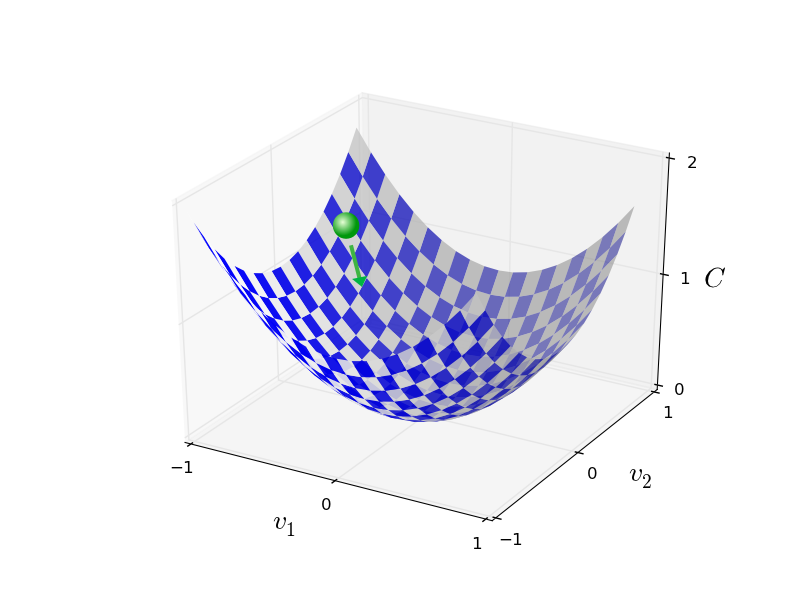
\includegraphics[width=.55\textwidth]{media_tesi/valley_with_ball.png}}
\caption{Il grafico della funzione $C(v_{1}, v_{2})$ con la pallina verde che rappresenta il punto in analisi e l'opposto del vettore gradiente spiccato in esso, ad indicare in quale direzione muoverebbe nella discesa}
\label{gradiente}
\end{figure}

Se ora abbiamo un'idea più chiara di cosa sia il vettore gradiente spieghiamo in cosa consiste il metodo della discesa che lo utilizza. Ipotizzando la stessa metafora della valle vogliamo sfruttare il fatto che la discesa della pallina si arresterà nella parte più bassa dalla depressione. Il nostro metodo computa una discesa simile ma diversa nel fatto che il percorso che farà la nostra pallina non approssimerà la discesa \textit{fisica} che avverrebbe nella realtà. Per cui il nostro metodo non si rifà alle equazioni della dinamica di Newton, è un pò diverso. Per ora sappiamo che, dato un punto sulla superficie di una valle, la direzione opposta a quella del gradiente è quella in cui la palla si muoverebbe se fosse libera di scendere; nel nostro metodo seguiamo un percorso di discesa fatto di tanti piccoli passi che prevedono, partendo da un punto, di muoversi verso $-\nabla C$ per un piccolo tratto. Mossi nel nuovo punto, che chiamiamo $P_{2}$, ricalcoleremmo il gradiente $\nabla C(P_{2})$ e faremmo un altro piccolo passo in direzione $- \nabla C(P_{2})$. Si capisce che questo metodo va iterato a lungo per scendere lungo la valle fino ad arrivare nel suo punto più basso. Tra un iterazione $k$ e la successiva $k+1$, ci saremo spostati dal punto $P_{k}$ al punto $P_{k+1}$ per cui $ \Delta P= P_{k+1}-P_{k}=-\eta \nabla C$ dove $\eta$ è un piccolo parametro positivo detto il \textit{learning rate} che fornisce un indicazione di quanto grande sia la distanza percorsa fra un iterazione e l'altra nell'algoritmo; va da se che se il $\eta$ cresce l'algoritmo procede più speditamente, ma questo potrebbe portare anche a degli errori. Ritorniamo dal parallelo con la valle, la palla e le variabili $v$ alla nostra funzione dei costi $C(w, b)$ e vediamo come il metodo del gradiente funzioni con più di due variabili, anche se di questa situazione non potremo avere una visualizzazione. Cosi come ci spostiamo da un punto all'altro nella valle, aggiornando le due variabili della nostra posizione, ora aggiorniamo le variabili della funzione dei costi, ovvero $w$ i pesi e $b$ i bias. Le regola per aggiornare queste componenti sarà:
\begin{equation}
w_{k}\rightarrow w'_{k}=w_{k}-\eta \dfrac{\partial C}{\partial w_{k}}
\end{equation}
\begin{equation}
b_{l}\rightarrow b'_{l}=b_{l}-\eta \dfrac{\partial C}{\partial b_{l}}
\end{equation}
dove $k$ e $l$ variano, rispettivamente, tra tutti i pesi e i bias della rete. Ripetendo questa regola arriveremo a trovare il minimo della funzione.
%\begin{center}
%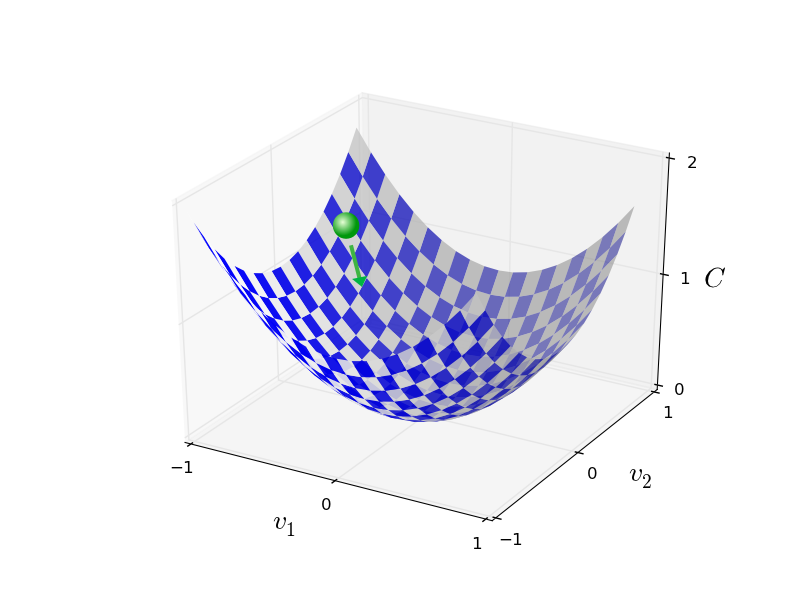
\includegraphics[width=0.5\textwidth]{media_tesi/valley_with_ball.png}
%\caption{Il grafico della funzione $C(v_{1}, v_{2})$ con la pallina verde che rappresenta il punto in analisi e il vettore gradiente spiccato da esso, ad indicare in quale direzione moverebbe nella discesa}
%\end{center}
\\
Ora che abbiamo spiegato come funziona il gradiente dobbiamo andare più a fondo a spiegare come interagiscono fra loro i neuroni collegati, come si attivano e come propagano il proprio segnale.
Ogni neurone $j^{th}$ è collegato (stiamo sempre parlando del caso delle reti feed forward) ai neuroni dello strato precedente dall'arco di peso $w^{l}_{jk}$ (cioè dal neurone $k$ in $l-1$ al neurone $j$ in $l$) e la sua attivazione viene determinata da una computazione fatta sui segnali in ingresso, più precisamente è la somma delle attivazioni dei neuroni dello stato precedente a lui collegati, moltiplicati per il peso del loro arco verso $j^{th}$ più una quantità $b_{j}$ specifica del neurone $j$ nello strato $l$, questa somma prende il nome di $z^{l}_{j}$. 

\begin{equation}
\displaystyle a^{l}_{j}=\sigma\left( z^{l}_{j}\right) = \sigma \left( \sum_{k}w^{l}_{jk}a^{l-1}_k +b^{l}_{j} \right)
\end{equation}

Spieghiamo brevemente cosa è $\sigma$. Ogni neurone riceve input dagli strati precedenti e internamente deve decidere se propagare a sua volta lo stimolo o meno. In biologia abbiamo già anticipato che i neuroni, una volta eccitati, non hanno una via di mezzo nel rispondere al segnale, per cui, o propagano a loro volta lo stimolo nella rete ``accendendosi''  oppure rimangono in quiete senza reagire. Nelle reti neurali la funzione di attivazione di solito non emette un segnale binario, piuttosto propaga vari livelli d'intensità del segnale. $\sigma$ rappresenta quella classe di funzioni sigmoidali che ben si adattano a rappresentare l'attivazione dei neuroni e che hanno lo scopo di normalizzare gli output nel range da $0$ a $1$. Quindi, se un neurone reale può veder rappresentata la propria funzione di attivazione come una funzione a gradino una sigmoide è la versione addolcita della funzione gradino, come mostriamo qui sotto con il plot della funzione sigmoide:
\begin{equation}
	\sigma(z)=\dfrac{1}{1+e^{-z}}
\end{equation}

%\begin{figure}[hbtb]
%\centering
%{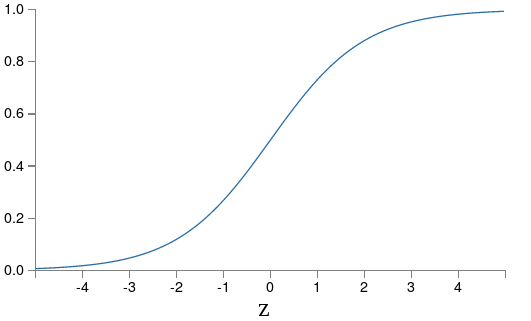
\includegraphics[width=.45\textwidth]{media_tesi/sigmoide.png}}
%\caption{Il grafico della funzione sigmoide $\sigma(z)$}
%\label{fig:subfig}
%\end{figure}

\begin{figure}[hbtb]
\centering
\subfloat[][\emph{Grafico della funzione sigmoide $\sigma(z)$}]
{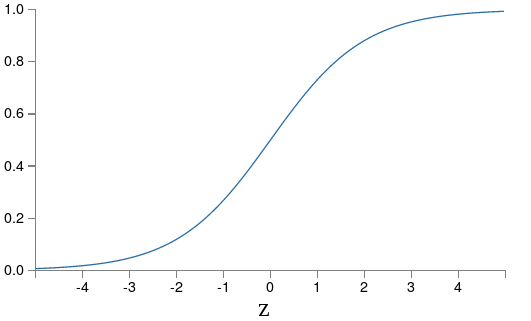
\includegraphics[width=.45\textwidth]{media_tesi/sigmoide.png}} \qquad
\subfloat[][\emph{Grafico ReLu}]
{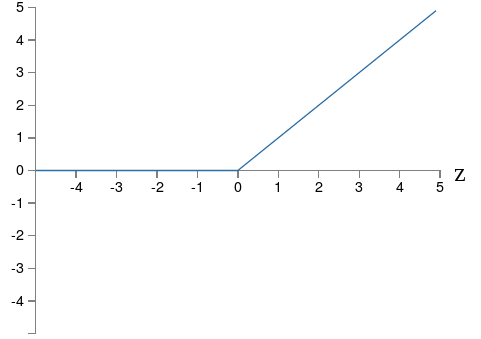
\includegraphics[width=.41\textwidth]{media_tesi/relu.png}} \\
\caption{Confronto tra due funzioni di attivazione}
\label{fig:subfig}
\end{figure}

La sigmoide non è l'unica funzione adatta per le reti neurali. Si usa anche $tanh$ oppure, un altra funzione è la \textit{ReLu}(Rectified Linear Unit)  $\displaystyle f(z)=max(0,z)$ che venne resa popolare quando la \textit{AlexNet} vinse la sfida \textit{ImageNet}nel 2012, un concorso che premia i migliori algoritmi per l'\textit{object detection} e la classificazione delle immagini. La \textit{AlexNet} usava \textit{ReLu} come funzione di attivazione e da quel momento in poi altri la adottarono ai propri scopi rendendosi conto, in via empirica, che funzionava meglio di quanto usato fino a quel momento \cite{krizhevsky2012imagenet}. Non è perfettamente chiaro cosa la renda migliore ma si pensa che la convergenza del metodo del gradiente venga velocizzata da \textit{ReLu} grazie alla sua semplicità e alla sua capacità di non saturarsi\cite{cs23}.

L'output di un neurone è denotato da $ a^{l}_{j} $ per ogni neurone $j$ nello strato $l$, possiamo definire un vettore contenente questi output per tutti gli $n$ neuroni di quello strato $a^{l} = \left[a^{l}_{1},a^{l}_{2}, \cdots, a^{l}_{j}, \cdots, a^{l}_{n}  \right] $. Vediamo ora come di strato in strato i neuroni si attivano fra loro e per questo adottiamo una notazione matriciale di quanto abbiamo appena visto: denotiamo allora una matrice $w^{l}$ dei pesi per ogni layer della rete, dove le sue entry sono $w^{l}_{kj}$ i vari pesi che legano i neuroni fra lo strato $l-1$ ed $l$ e denotiamo, allo stesso modo di $a^{l}$ anche il vettore dei \textit{bias} $b^{l}$ per il livello $l$ e riscriviamo la formula 3 come:
\begin{equation}
	a^{l}=\sigma\left( w^{l}a^{l-1}+b^{l}\right)
\end{equation}
\\
La propagazione del calcolo degli output dei singoli livelli procede verso il livello finale, l'\textit{output layer}, e una volta calcolato l'errore nella funzione dei costi, $C$, questo errore viene propagato in senso opposto fino al layer degli input. Spieghiamo meglio quale è il senso di questo ``propagarsi''. 
$C(w,b)$ è stata definita in (1) e viene calcolata sull'output layer $a$ della rete, questo che possiamo indicare per chiarezza come $a^{out}$ per esplicitare a quale livello sia riferito è calcolato a sua volta come indicato nella (5) ed   è quindi funzione dei pesi e dei bias del livello che lo precedono: $ a^{out}(w^{l},b^{l}, a^{l})$ dove $l$ è l'ultimo \textit{hidden layer}, quello prima di \textit{out}; ma compare anche $a^{l}$, questo in catena è una funzione di pesi, attivazioni e bias di $l-1$. Vediamo quindi come in verità tutta la funzione dei costi non sia altro che una lunghissima e imponente funzione composta, che richiama i parametri dei livelli sottostanti. Compreso questo possiamo dire che se la $C$ è una funzione composta dei pesi e dei bias di tutti i suoi sottolivelli e quindi della rete in generale; possiamo cercare di capire in che modo questi parametri, lungo la rete, contribuiscano alla definizione di $C$ e in ultima analisi di come contribuiscano alla quantità dell'errore espresso da $C$ e della rete nel suo complesso; in questo senso l'errore viene retropropagato lungo la rete. Per vedere che peso ha complessivamente un peso $w_{k}^{l}$ si calcola la sua derivata parziale $\frac{\partial C}{\partial w_{k}^{l}}$ ma per poter far questo bisogna procedere livello per livello. Abbiamo detto che $C$ è una funzione composta ed è necessario partire livello di output e andare indietro per calcolare le derivate dei pesi più in profondità applicando la \textit{chain rule} delle funzioni composte $(f \circ g)'=(f' \circ g) \cdot g' $.
\begin{equation}
	C(a^{out})= C( a^{out}(w^{l},b^{l}, a^{l})) = C( a^{out}(w^{l},b^{l}, a^{l}(w^{l-1},b^{l-1}, a^{l-1}))) = \cdots
\end{equation}
La formula sopra dovrebbe rendere l'idea di come si procede a comporre la funzione costi, innestando via via i pesi e i bias. Per trovare la derivata $\frac{\partial C}{\partial w_{k}^{m}} $ di un peso di un neurone nel livello $m$ dovremo quindi calcolare prima di lui tutte le derivate delle funzioni che lo contengono:
\begin{equation}
	\dfrac{\partial C}{\partial w_{k}^{m}} = \dfrac{\partial C}{\partial a^{out}}\cdot \dfrac{\partial a^{out}}{\partial a^{l-1}} \cdot \dfrac{\partial a^{l-1}}{\partial a^{l-2}}\cdot \; \cdots \; \cdot \dfrac{\partial a^{m}}{\partial w^{m}_{k}}
\end{equation} 
In questo senso la procedura avanza verso la base della rete, calcolando tutte le derivate parziali rispetto ai $w$ e ai $b$ della rete (per ogni neurone di ogni layer); il che corrisponde ad avere calcolato il gradiente della funzione dei costi:
\begin{equation}
	\nabla C = \left[ \dfrac{\partial C}{\partial w_{1}^{1}}, \dfrac{\partial C}{\partial w_{2}^{1}}, \cdots, \dfrac{\partial C}{\partial w_{n}^{1}},\dfrac{\partial C}{\partial b_{1}^{2}}, \cdots \dfrac{\partial C}{\partial b_{2}^{2}}, \cdots \right] 
\end{equation} 
Una volta ottenuto il gradiente di $C$ possiamo procedere all'aggiornamento dei pesi, l'apprendimento della rete si basa infatti su questo, sulla modifica dei suoi parametri interni in modo che dal loro cambiamento scaturisca un comportamento complessivamente diverso (migliore) nei confronti degli input che le vengono passati e con diversi training riesca a darci i risultati che speriamo.
La regola di aggiornamento di un generico peso è questa:
\begin{equation}
	w_{j}^{l +} = w_{j}^{l} + \eta \dfrac{\partial C}{\partial w_{j}^{l}}
\end{equation}
che altro non è che la procedura della discesa del gradiente spiegata in precedenza.

\section{I miglioramenti}
\subsection*{Migliorare backpropagation attraverso diversi approcci sulla discesa del gradiente}

L'algoritmo di backpropagation si basa sull'ottimizzazione di una funzione d'errore tra l'output della rete e il risultato desiderato. La funzione in questione ha come variabili i pesi associati ai collegamenti tra i vari neuroni della rete e i loro bias. Nella sua versione più semplice la funzione cerca il proprio minimo seguendo la direzione del proprio gradiente.
Venendo alle variazioni su questo metodo; furono proposti il \textit{metodo dei minimi quadrati} (in inglese OLS: Ordinary Least Squares) e il \textit{metodo detto di quasi-newton} (che è una variazione sul canonico metodo di Newton) che risultano essere però troppo lenti da computare, in special modo nelle reti molto ampie e ad entrare nello specifico il problema per i metodi di quasi-newton è che lo spazio in memoria richiesto per salvare una approssimazione dell'inversa dell'Hessiana cresce quadraticamente rispetto al numero dei pesi su cui viene effettuato il calcolo \cite{saito1997partial}. Altre tecniche come \textit{BFGS} o il \textit{gradiente coniugato} possono essere in alcuni casi delle valide alternative.
Più genericamente il problema del migliorare l'ottimizzazione dell'errore trova soluzione quando si migliora la capacità di computare la più utile lunghezza di passo possibile (step-lenght) ovvero quanto distante una iterazione deve essere da quella che la precede avendo seguito la direzione del gradiente.
Esistono per questo algoritmi del secondo ordine e del primo ordine, che possiamo vedere a confronto nelle due immagini in Figura \ref{discese}.

\vspace{5 mm}

\begin{figure}[hbtb]
\centering
\subfloat[][\emph{Traiettorie algoritmi del primo ordine}]
{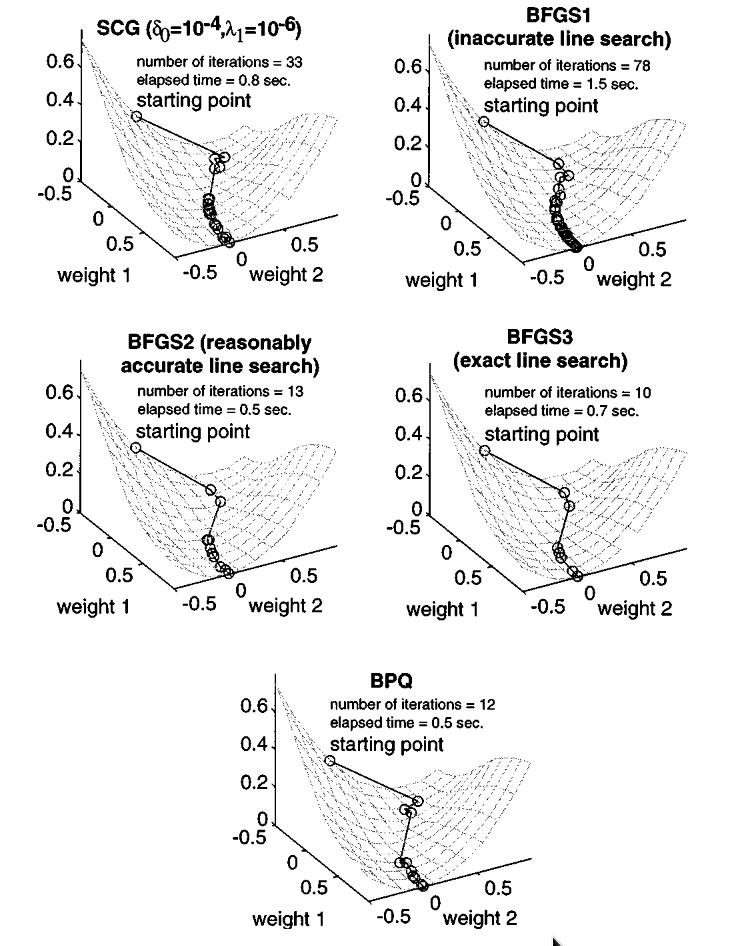
\includegraphics[width=.45\textwidth]{media_tesi/learning_trajectories_of_second_order.jpeg}} \quad
\subfloat[][\emph{Traiettorie algoritmi del secondo ordine}]
{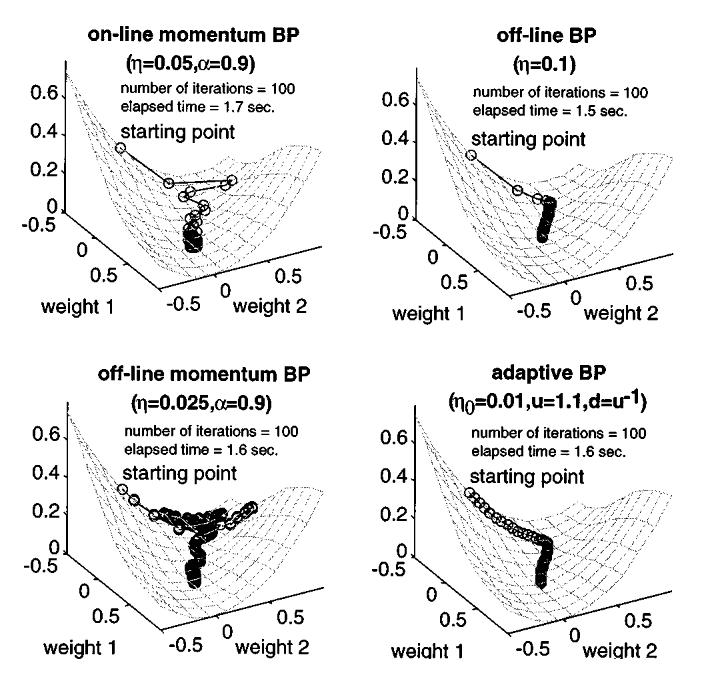
\includegraphics[width=.45\textwidth]{media_tesi/learning_trajectories_of_first_order.jpeg}} \\
\caption{Confronto tra tipologie diverse di algoritmi}
\label{discese}
\end{figure}
\vspace{5 mm}

Si può vedere come l'andamento della traiettoria conduca al minimo in numero inferiori di passi utilizzando algoritmi del secondo ordine.

Per velocizzare BP è stato anche introdotto il momento, che ha lo scopo di ridurre le oscillazioni della traiettoria dovute ad una non proficua scelta della lunghezza del passo per le iterazioni e fu proprio nel 1988 che Robert A. Jacobs, propose quattro euristiche per il miglioramento del tasso di convergenza del backpropagation \cite{nielsen_book}.

Nel 1988 la ricerca aveva già riconosciuto la bontà della procedura BP e si investigavano quegli algoritmi di ricerca dell'ottimo per la funzione di minimo che computassero la discesa del gradiente soltanto localmente (ovvero rimanendo in intorni molto vicini al punto di iterazione). Questo cosidetto \textit{locality constraint} veniva motivato dal fatto che costituiva una buona metafora tecnologica della controparte biologica, le reti neurali, a cui si ispirava e in secondo luogo dall'ipotesi che questi algoritmi \textit{locali} fossero più adatti ad essere processati in parallelo.
Fra le quattro euristiche di Jacobs vi era l'adattamento dei tassi d'apprendimento nel tempo e si spiega che ogni peso della rete dovrebbe avere il proprio tasso d'apprendimento specifico. Le implementazioni di queste euristiche venivano individuate nel \textit{momento} e nella regola d'apprendimento \textit{delta-bar-delta}.
\subsection*{Low complexity NNs}
Alcuni altri indirizzi di miglioramento dell'efficacia delle reti sfruttano il BP per modellare delle reti meno complesse (\textit{low complexity}) che possano essere utili a scopi meno sofisticati. Ad esempio, nelle reti convuluzionali, dove il processo di riconoscimento degli oggetti ha luogo, gli algoritmi vengono eseguiti su GPU che dissipano grandi quantità di energia e un tale scenario non è adatto a scopi dove il livello di dettaglio nel riconoscere gli oggetti non è così elevato. Applicazioni più popolari e frequenti come il riconoscimento facciale nei dispositivi mobili deve per forza di cose girare in locale sui processori embedded che animano gli smartphone, per questo i ricercatori sfruttano varianti del BP per creare reti convuluzionali a bassa complessità. Queste modellano problemi che richiedono meno risorse e possono quindi essere eseguite più velocemente anche sui dispositivi meno prestanti\cite{TSD}.
\subsection*{Le performance con CPU e GPU}
Nella sezione riguardante la matematica di backpropagation abbiamo citato come i calcoli per le attivazioni dei neuroni non vengano eseguiti uno alla volta ma, livello per livello, vengano raggruppati in vettori e matrici non solo per snellire la notazione usata ma anche perché a tutti gli effetti è quello che accade realmente. La quantità di dati coinvolta in una rete neurale può essere davvero notevole, con lo strato di input che può avere fino a migliaia di nodi, per questo le matrici che vengono coinvolte nei calcoli possono diventare molto grandi ed occupare notevoli quantità di spazio in memoria.\\ 

Tale utilizzo di memoria costituisce un limite difficile per la computazione da parte delle CPU, anche quelle multi-core. Le CPU ottimizzano la velocità di calcolo sui singoli processi seriali e sono un'alternativa ad un altro tipo di architettura per processori: le GPU. Le GPU furono inventate a detta di Nvidia nel 1999 ma le loro origini risalgono a molti anni prima e datare un nascita per questa tecnologia è quasi impossibile visto che deriva dall'evoluzione di soluzioni tecnologiche affini per scopi che si sono succedute nel corso degli anni. Nel 2007 gli sviluppatori poterono sfruttare le potenzialità di calcolo parallelo anche per applicazioni più generiche grazie alla piattaforma di programmazione \textit{CUDA}. Nel 2009 un documento accademico di Stanford illustrava quanto più velocemente si potesse addestrare delle reti neurali utilizzando metodi con GPU, fino a 70 volte più veloci della controparte con CPU \cite{raina2009large}. Tale approccio consentì l'uso di dataset più ricchi e un aumento dei parametri a disposizione per settare la rete. 

Ma perchè le GPU? Tanta più memoria si necessita per sviluppare i calcoli di queste matrici tanto più l'utilizzo delle GPU migliora le prestazione perché consiste di numerose unità di calcolo semplici che possono agire in parallelo.
\\
Un esperimento presentato da alcuni studiosi nel 2016 comparava due reti neurali nello svolgere il medesimo compito, una implementata su GPU l'altra su CPU. L'esperimento consiste nel riconoscere cifre numeriche scritte a mano, presentate in un dataset chiamato \textit{MNIST}, come quelle in Figura \ref{MNIST}. Presentiamo i risultati delle velocità di computazione nella tabella e nel grafico riportato sotto, dai quali possiamo evidenziare come aver allenato la rete neurale attraverso la GPU aumenti di un fattore molto grande le performance rispetto alla controparte in CPU e che la GPU sia da preferire quando nella rete sono presenti un grande numero di attributi, altrimenti il costo dell'inizializzazione della scheda non verrebbe giustificato dall'incremento delle velocità \cite{brito2016gpu}.

\vspace{15mm}

\begin{figure}[h]
\centering
{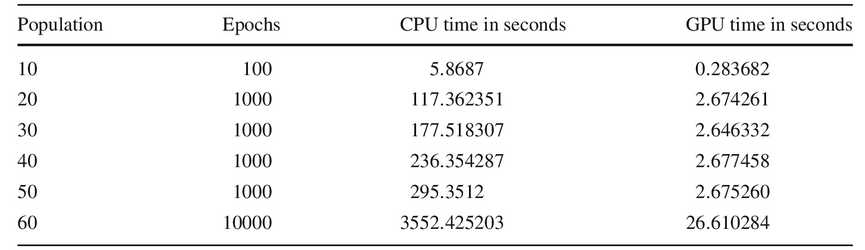
\includegraphics[scale=0.65]{media_tesi/table_experiment.png}}
\caption{Riassunto dei risultati dell'esperimento \cite{brito2016gpu}}
\label{fig:subfig}
\end{figure}

\begin{figure}[h]
\centering
{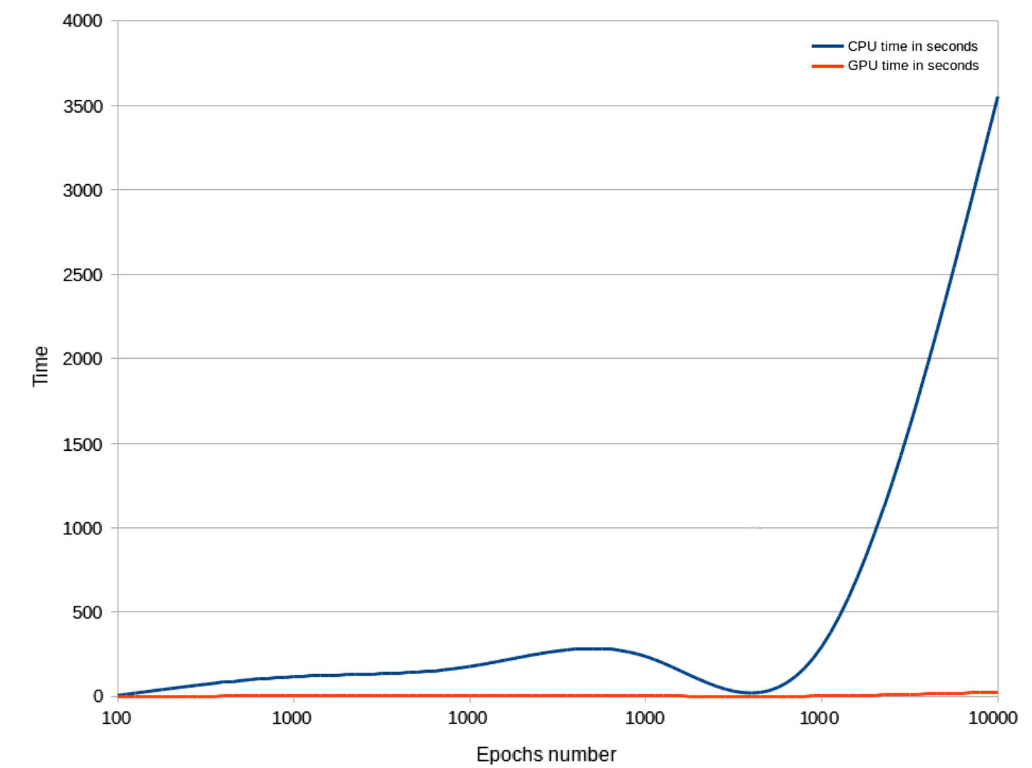
\includegraphics[scale=0.5]{media_tesi/graph_GPU_vs_CPU.png}}
\caption{Il grafico che mostra le differenze tra le velocità di esecuzione tra CPU e GPU \cite{brito2016gpu}}
\label{fig:subfig}
\end{figure}

\begin{figure}[b]
\centering
{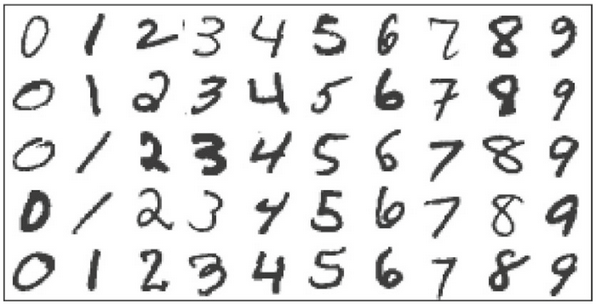
\includegraphics[scale=0.5]{media_tesi/MNIST.png}}
\caption{Un esempio di cifre da riconoscere da parte della reti nell'esperimento}
\label{MNIST}
\end{figure}

%\begin{figure}[hbtb]
%\centering
%\subfloat[][\emph{Traiettorie algoritmi del primo ordine}]
%{\includegraphics[width=.45\textwidth]{media_tesi/}} \quad
%\subfloat[][\emph{Traiettorie algoritmi del secondo ordine}]
%{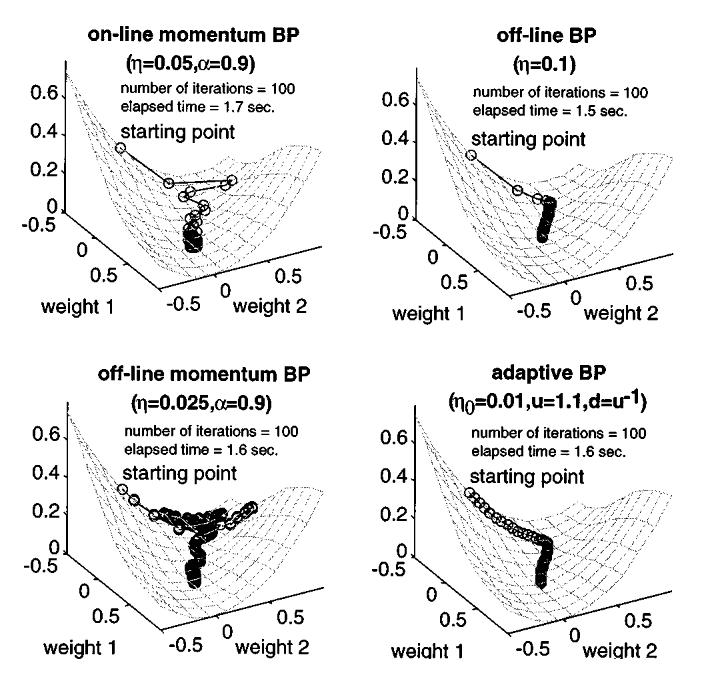
\includegraphics[width=.45\textwidth]{media_tesi/learning_trajectories_of_first_order.jpeg}} \\
%\caption{Confronto tra tipologie diverse di algoritmi}
%\label{fig:subfig}
%\end{figure}
